% !TeX spellcheck = en_US
%#------------------------------------------------------------------------------
%# Name:        OpenGeoHub-machine-learning-training.Rnw
%#              (knitr document: R + Latex)
%#
%# Inhalt:      Exercises for OpenGeoHub Summer School, 1. Series
%#
%# Autorin:     Madlene Nussbaum, BFH-HAFL
%# Datum:       August 2018
%# Licence:     GNU General Public License
%#------------------------------------------------------------------------------

\documentclass[11pt,a4paper,twoside]{article}\usepackage[]{graphicx}\usepackage[]{color}
% maxwidth is the original width if it is less than linewidth
% otherwise use linewidth (to make sure the graphics do not exceed the margin)
\makeatletter
\def\maxwidth{ %
  \ifdim\Gin@nat@width>\linewidth
    \linewidth
  \else
    \Gin@nat@width
  \fi
}
\makeatother

\definecolor{fgcolor}{rgb}{0.345, 0.345, 0.345}
\newcommand{\hlnum}[1]{\textcolor[rgb]{0.686,0.059,0.569}{#1}}%
\newcommand{\hlstr}[1]{\textcolor[rgb]{0.192,0.494,0.8}{#1}}%
\newcommand{\hlcom}[1]{\textcolor[rgb]{0.678,0.584,0.686}{\textit{#1}}}%
\newcommand{\hlopt}[1]{\textcolor[rgb]{0,0,0}{#1}}%
\newcommand{\hlstd}[1]{\textcolor[rgb]{0.345,0.345,0.345}{#1}}%
\newcommand{\hlkwa}[1]{\textcolor[rgb]{0.161,0.373,0.58}{\textbf{#1}}}%
\newcommand{\hlkwb}[1]{\textcolor[rgb]{0.69,0.353,0.396}{#1}}%
\newcommand{\hlkwc}[1]{\textcolor[rgb]{0.333,0.667,0.333}{#1}}%
\newcommand{\hlkwd}[1]{\textcolor[rgb]{0.737,0.353,0.396}{\textbf{#1}}}%
\let\hlipl\hlkwb

\usepackage{framed}
\makeatletter
\newenvironment{kframe}{%
 \def\at@end@of@kframe{}%
 \ifinner\ifhmode%
  \def\at@end@of@kframe{\end{minipage}}%
  \begin{minipage}{\columnwidth}%
 \fi\fi%
 \def\FrameCommand##1{\hskip\@totalleftmargin \hskip-\fboxsep
 \colorbox{shadecolor}{##1}\hskip-\fboxsep
     % There is no \\@totalrightmargin, so:
     \hskip-\linewidth \hskip-\@totalleftmargin \hskip\columnwidth}%
 \MakeFramed {\advance\hsize-\width
   \@totalleftmargin\z@ \linewidth\hsize
   \@setminipage}}%
 {\par\unskip\endMakeFramed%
 \at@end@of@kframe}
\makeatother

\definecolor{shadecolor}{rgb}{.97, .97, .97}
\definecolor{messagecolor}{rgb}{0, 0, 0}
\definecolor{warningcolor}{rgb}{1, 0, 1}
\definecolor{errorcolor}{rgb}{1, 0, 0}
\newenvironment{knitrout}{}{} % an empty environment to be redefined in TeX

\usepackage{alltt}

\usepackage[utf8]{inputenc}
\usepackage{blindtext} % for blind text
\usepackage{hyperref} % links in table of contents
\usepackage[english]{babel}
\usepackage{amsthm} % for renvironment
\usepackage{natbib}
\usepackage[iso,german]{isodate}
\usepackage{subcaption}

\newtheorem{rexample}{R Example}[section]

% Some colors for the links
\definecolor{darkblue}{rgb}{0,0,0.5}
\definecolor{darkmagenta}{rgb}{0.5,0,0.5}
\definecolor{darkgreen}{rgb}{0,0.4,0}
\definecolor{darkred}{rgb}{0.7,0,0}

\hypersetup{
draft=false,
colorlinks=true,linkcolor=darkblue,citecolor=darkred,urlcolor=darkgreen,
breaklinks=true, bookmarksnumbered=true
}

% % Headers
\usepackage{fancyhdr}
\pagestyle{fancy}
\fancyhf{}
\fancyhead[OL]{\leftmark}% odd page, left
\fancyhead[OR]{\thepage}% odd page, right
\fancyhead[EL]{\thepage}% even page, left 
\fancyhead[ER]{\leftmark}% even page, right
\renewcommand{\headrulewidth}{0.4pt}
\fancyheadoffset[R]{1pt}

% captions in bold
\usepackage[font = {small}, labelfont = bf]{caption}

% format page borders
\usepackage[a4paper]{geometry}
\geometry{verbose,tmargin=2.5cm,bmargin=2.3cm,lmargin=2.5cm,rmargin=3cm,headheight=1.7cm,headsep=0.9cm,footskip=1.5cm}

% no indents
\setlength\parindent{0pt}
\setlength{\parskip}{3pt}


% Top aling logos on title page
\def\imagebox#1#2{\vtop to #1{\null\hbox{#2}\vfill}}

\newcommand{\bskip}{\vspace{0.7cm}}
\IfFileExists{upquote.sty}{\usepackage{upquote}}{}
\begin{document}

% % Logos
\begin{figure}
\centering
\begin{subfigure}[t]{0.27\textwidth}
% 
\includegraphics[width=\textwidth]{BFH-Logo.pdf}
\imagebox{37.5mm}{
\includegraphics[width=\textwidth]{figure/BFH-Logo.pdf}}
\end{subfigure}
\hfill
\begin{subfigure}[t]{0.3\textwidth}
% \includegraphics[width=\textwidth]{3455_original_isric.png}
\imagebox{37.5mm}{
\includegraphics[width=\textwidth]{figure/logo-opengeohub.png}}
\end{subfigure}
\end{figure}

% Title
\vspace{5cm}
{\LARGE\textsf{OpenGeoHub Summer School}}

\vspace{0.7cm}
{\Large\textbf{\textsf{Mastering Machine Learning for Spatial Prediction I} }}

\vspace{0.3cm}

{\Large\textsf{Practical training}  }

\vspace{0.5cm}
\textsf{Madlene Nussbaum, 4/5 September 2019}

{ \small \textsf{\copyright~ CC-BY-NC-SA } 	} 
\bigskip


% Table of contents (with empty back page()
\setlength{\parskip}{0pt}
\tableofcontents
\thispagestyle{empty}
\setlength{\parskip}{4pt}

% \newpage
% \mbox{}
% \thispagestyle{empty}
% \newpage

% --------






\section*{Preparation}

Load needed packages:

\begin{knitrout}
\definecolor{shadecolor}{rgb}{0.969, 0.969, 0.969}\color{fgcolor}\begin{kframe}
\begin{alltt}
\hlcom{# install.packages(c("grpgreg", "glmnet", "kernlab", "caret", "randomForest", "mboost",}
\hlcom{#                    "gbm", "geoGAM", "raster"))}
\hlkwd{library}\hlstd{(grpreg)} \hlcom{# for grouped lasso}
\hlkwd{library}\hlstd{(glmnet)} \hlcom{# for general lasso}
\hlkwd{library}\hlstd{(kernlab)} \hlcom{# for support vector machines}
\hlkwd{library}\hlstd{(caret)} \hlcom{# for model tuning}
\hlkwd{library}\hlstd{(randomForest)} \hlcom{# to fit random forest}
\hlkwd{library}\hlstd{(mboost)} \hlcom{# for the boosting models with linear and spline terms  }
\hlkwd{library}\hlstd{(gbm)} \hlcom{# for the boosting model with trees}
\hlkwd{library}\hlstd{(geoGAM)} \hlcom{# for the berne dataset}
\hlkwd{library}\hlstd{(raster)} \hlcom{# for plotting as a raster}
\hlkwd{library}\hlstd{(parallel)} \hlcom{# for parallel computing}
\end{alltt}
\end{kframe}
\end{knitrout}

As an example you can work with the Berne soil mapping study area: dataset \texttt{berne} in R package \texttt{geoGAM}, contains continuous, binary and a multinomial/ordered response and a spatial data \texttt{berne.grid} for prediction. 

Feel free to work with your own data!

Hint: The processing of this code is quite time consuming on a laptop. Normaly, one uses high performance computing facilities for machine learning.  

Load the data, select the calibration set and remove missing values in covariates: 

\begin{knitrout}
\definecolor{shadecolor}{rgb}{0.969, 0.969, 0.969}\color{fgcolor}\begin{kframe}
\begin{alltt}
\hlkwd{data}\hlstd{(berne)}
\hlkwd{dim}\hlstd{(berne)}
\end{alltt}
\begin{verbatim}
## [1] 1052  238
\end{verbatim}
\begin{alltt}
\hlcom{# Continuous response }
\hlstd{d.ph10} \hlkwb{<-} \hlstd{berne[berne}\hlopt{$}\hlstd{dataset} \hlopt{==} \hlstr{"calibration"} \hlopt{& !}\hlkwd{is.na}\hlstd{(berne}\hlopt{$}\hlstd{ph.0.10), ]}
\hlstd{d.ph10} \hlkwb{<-} \hlstd{d.ph10[}\hlkwd{complete.cases}\hlstd{(d.ph10[}\hlnum{13}\hlopt{:}\hlkwd{ncol}\hlstd{(d.ph10)]), ]}
\hlcom{# select validation data for subsequent validation}
\hlstd{d.ph10.val} \hlkwb{<-} \hlstd{berne[berne}\hlopt{$}\hlstd{dataset} \hlopt{==} \hlstr{"validation"} \hlopt{& !}\hlkwd{is.na}\hlstd{(berne}\hlopt{$}\hlstd{ph.0.10), ]}
\hlstd{d.ph10.val} \hlkwb{<-} \hlstd{d.ph10.val[}\hlkwd{complete.cases}\hlstd{(d.ph10.val[}\hlnum{13}\hlopt{:}\hlkwd{ncol}\hlstd{(d.ph10)]), ]}
\hlcom{# Binary response }
\hlstd{d.wlog100} \hlkwb{<-} \hlstd{berne[berne}\hlopt{$}\hlstd{dataset}\hlopt{==}\hlstr{"calibration"}\hlopt{&!}\hlkwd{is.na}\hlstd{(berne}\hlopt{$}\hlstd{waterlog.100), ]}
\hlstd{d.wlog100} \hlkwb{<-} \hlstd{d.wlog100[}\hlkwd{complete.cases}\hlstd{(d.wlog100[}\hlnum{13}\hlopt{:}\hlkwd{ncol}\hlstd{(d.wlog100)]), ]}
\hlcom{# Ordered/multinomial tesponse }
\hlstd{d.drain} \hlkwb{<-} \hlstd{berne[berne}\hlopt{$}\hlstd{dataset} \hlopt{==} \hlstr{"calibration"} \hlopt{& !}\hlkwd{is.na}\hlstd{(berne}\hlopt{$}\hlstd{dclass), ]}
\hlstd{d.drain} \hlkwb{<-} \hlstd{d.drain[}\hlkwd{complete.cases}\hlstd{(d.drain[}\hlnum{13}\hlopt{:}\hlkwd{ncol}\hlstd{(d.drain)]), ]}
\hlcom{# covariates start at col 13}
\hlstd{l.covar} \hlkwb{<-} \hlkwd{names}\hlstd{(d.ph10[,} \hlnum{13}\hlopt{:}\hlkwd{ncol}\hlstd{(d.ph10)])}
\end{alltt}
\end{kframe}
\end{knitrout}



\section{Lasso -- linear shrinkage method}
\markboth{Lasso -- linear shrinkage method}{Lasso -- linear shrinkage method}

\paragraph{Lasso for continuous response} \mbox{}  \nolinebreak

The \texttt{berne} dataset contains categorical covariates (factors, e.g. geological map with different substrate classes). The group lasso (R package \texttt{grpreg}) ensures that all dummy covariates of one factor are excluded (coefficients set to 0) together or remain in the model as a group.

The main tuning parameter $\lambda$ is selected by cross validation. $\lambda$ determines the degree of shrinkage that is applied to the coefficients. 


\bigskip 

HINT for R newbies: the \texttt{apply}-functions in R are replacements for loops (\texttt{sapply}: loop over a sequence of numbers, \texttt{lapply}: loop over a list). Compared to \texttt{for}, an \texttt{apply} is much faster and general coding style, though a bit more tricky to program. 

Example, how to replace a \texttt{for} by a \texttt{sapply}: 
\begin{knitrout}
\definecolor{shadecolor}{rgb}{0.969, 0.969, 0.969}\color{fgcolor}\begin{kframe}
\begin{alltt}
\hlcom{# loop }
\hlcom{# first create a vector to save the results}
\hlstd{t.result} \hlkwb{<-} \hlkwd{c}\hlstd{()}
\hlkwa{for}\hlstd{( ii} \hlkwa{in} \hlnum{1}\hlopt{:}\hlnum{10} \hlstd{)\{ t.result} \hlkwb{<-} \hlkwd{c}\hlstd{(t.result, ii}\hlopt{^}\hlnum{2}\hlstd{) \}}
\hlcom{# the same as apply}
\hlstd{t.result} \hlkwb{<-} \hlkwd{sapply}\hlstd{(}\hlnum{1}\hlopt{:}\hlnum{10}\hlstd{,} \hlkwa{function}\hlstd{(}\hlkwc{ii}\hlstd{)\{ ii}\hlopt{^}\hlnum{2} \hlstd{\})}
\hlcom{# of course, this example is even shorter using:}
\hlstd{t.result} \hlkwb{<-} \hlstd{(}\hlnum{1}\hlopt{:}\hlnum{10}\hlstd{)}\hlopt{^}\hlnum{2}
\end{alltt}
\end{kframe}
\end{knitrout}


Now we create the setup using \texttt{apply} and fit the grouped lasso:
\begin{knitrout}
\definecolor{shadecolor}{rgb}{0.969, 0.969, 0.969}\color{fgcolor}\begin{kframe}
\begin{alltt}
\hlcom{# define groups: dummy coding of a factor is treated as group}
\hlcom{# find factors}
\hlstd{l.factors} \hlkwb{<-} \hlkwd{names}\hlstd{(d.ph10[l.covar])[}
  \hlstd{t.f} \hlkwb{<-} \hlkwd{unlist}\hlstd{(} \hlkwd{lapply}\hlstd{(d.ph10[l.covar], is.factor) ) ]}
\hlstd{l.numeric} \hlkwb{<-}  \hlkwd{names}\hlstd{(t.f[} \hlopt{!}\hlstd{t.f ])}

\hlcom{# create a vector that labels the groups with the same number  }
\hlstd{g.groups} \hlkwb{<-} \hlkwd{c}\hlstd{(} \hlnum{1}\hlopt{:}\hlkwd{length}\hlstd{(l.numeric),}
               \hlkwd{unlist}\hlstd{(}
                 \hlkwd{sapply}\hlstd{(}\hlnum{1}\hlopt{:}\hlkwd{length}\hlstd{(l.factors),} \hlkwa{function}\hlstd{(}\hlkwc{n}\hlstd{)\{}
                   \hlkwd{rep}\hlstd{(n}\hlopt{+}\hlkwd{length}\hlstd{(l.numeric),} \hlkwd{nlevels}\hlstd{(d.ph10[, l.factors[n]])}\hlopt{-}\hlnum{1}\hlstd{)}
                 \hlstd{\})}
               \hlstd{)}
\hlstd{)}
\hlcom{# grpreg needs model matrix as input}
\hlstd{XX} \hlkwb{<-} \hlkwd{model.matrix}\hlstd{(} \hlopt{~}\hlstd{., d.ph10[,} \hlkwd{c}\hlstd{(l.numeric, l.factors), F])[,}\hlopt{-}\hlnum{1}\hlstd{]}

\hlcom{# cross validation (CV) to find lambda}
\hlstd{ph.cvfit} \hlkwb{<-} \hlkwd{cv.grpreg}\hlstd{(}\hlkwc{X} \hlstd{= XX,} \hlkwc{y} \hlstd{= d.ph10}\hlopt{$}\hlstd{ph.0.10,}
                      \hlkwc{group} \hlstd{= g.groups,}
                      \hlkwc{penalty} \hlstd{=} \hlstr{"grLasso"}\hlstd{,}
                      \hlkwc{returnY} \hlstd{= T)} \hlcom{# access CV results}
\end{alltt}
\end{kframe}
\end{knitrout}


Compute predictions for the validation set with optimal number of groups chosen by lasso:
\begin{knitrout}
\definecolor{shadecolor}{rgb}{0.969, 0.969, 0.969}\color{fgcolor}\begin{kframe}
\begin{alltt}
\hlcom{# choose optimal lambda: CV minimum error + 1 SE (see glmnet)}
\hlstd{l.se} \hlkwb{<-} \hlstd{ph.cvfit}\hlopt{$}\hlstd{cvse[ ph.cvfit}\hlopt{$}\hlstd{min ]} \hlopt{+} \hlstd{ph.cvfit}\hlopt{$}\hlstd{cve[ ph.cvfit}\hlopt{$}\hlstd{min ]}
\hlstd{idx.se} \hlkwb{<-} \hlkwd{min}\hlstd{(} \hlkwd{which}\hlstd{( ph.cvfit}\hlopt{$}\hlstd{cve} \hlopt{<} \hlstd{l.se ) )} \hlopt{-} \hlnum{1}

\hlcom{# create model matrix for validation set}
\hlstd{newXX} \hlkwb{<-} \hlkwd{model.matrix}\hlstd{(} \hlopt{~}\hlstd{., d.ph10.val[,} \hlkwd{c}\hlstd{(l.factors, l.numeric), F])[,}\hlopt{-}\hlnum{1}\hlstd{]}
\hlstd{t.pred.val} \hlkwb{<-}  \hlkwd{predict}\hlstd{(ph.cvfit,} \hlkwc{X} \hlstd{= newXX,}
                       \hlkwc{type} \hlstd{=} \hlstr{"response"}\hlstd{,}
                       \hlkwc{lambda} \hlstd{=  ph.cvfit}\hlopt{$}\hlstd{lambda[idx.se])}
\hlcom{# get CV predictions, e.g. to compute R2}
\hlstd{ph.lasso.cv.pred} \hlkwb{<-} \hlstd{ph.cvfit}\hlopt{$}\hlstd{Y[,idx.se]}
\end{alltt}
\end{kframe}
\end{knitrout}

Get the lasso (non-zero) coefficients of the optimal model:
\begin{knitrout}
\definecolor{shadecolor}{rgb}{0.969, 0.969, 0.969}\color{fgcolor}\begin{kframe}
\begin{alltt}
\hlcom{# get the non-zero coefficients:}
\hlstd{t.coef} \hlkwb{<-} \hlstd{ph.cvfit}\hlopt{$}\hlstd{fit}\hlopt{$}\hlstd{beta[, idx.se ]}
\hlstd{t.coef[ t.coef} \hlopt{>} \hlnum{0} \hlstd{]}
\end{alltt}
\begin{verbatim}
##                (Intercept)                 cl_mt_gh_4 
##               1.920227e+00               6.344935e-03 
##               tr_se_curv2m   tr_se_curvplan2m_std_10c 
##               9.734395e-05               1.716402e-02 
##   tr_se_curvplan2m_std_25c   tr_se_curvplan2m_std_50c 
##               1.714450e-02               2.037167e-03 
##                  tr_vdcn25          timesetd1979_2010 
##               1.064009e-03               1.337349e-01 
##    timesetd1968_1974_field ge_geo500h3idTorfbedeckung 
##               2.626367e-01               1.061680e-01
\end{verbatim}
\end{kframe}
\end{knitrout}



\begin{knitrout}
\definecolor{shadecolor}{rgb}{0.969, 0.969, 0.969}\color{fgcolor}\begin{figure}

{\centering 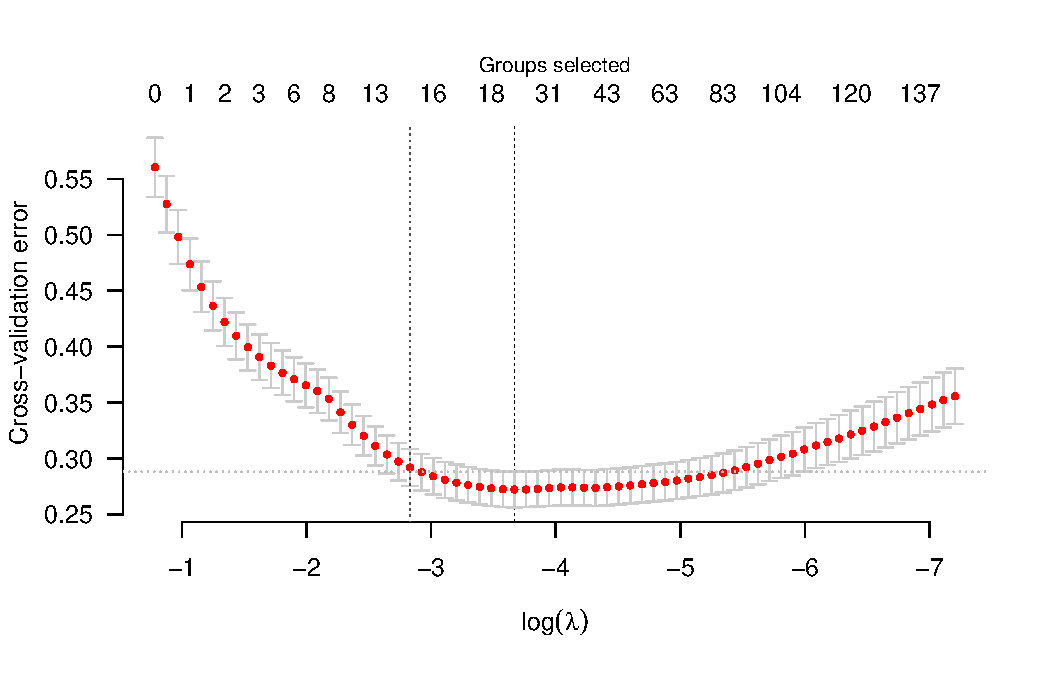
\includegraphics[width=0.8\textwidth]{figure/lasso-plot-cv-1} 

}

\caption[Cross validation error plotted against the tuning parameter lambda]{Cross validation error plotted against the tuning parameter lambda. The dashed line indicates lambda at minimal error, the dotted darkgrey line is the optimal lambda with minimal error + 1 SE.}\label{fig:lasso-plot-cv}
\end{figure}


\end{knitrout}


\paragraph{Lasso for multinomial response} \mbox{} \nolinebreak

I am not aware of a lasso implementation for multinomial responses 
that can handle groups of factors. Therefore, we use ``standard'' lasso from R package \texttt{glmnet} (the option \texttt{type.multinomial = "grouped"} does only ensure all coefficients of the multinomial model for the same covariate are treated as groups). 


\begin{knitrout}
\definecolor{shadecolor}{rgb}{0.969, 0.969, 0.969}\color{fgcolor}\begin{kframe}
\begin{alltt}
\hlcom{# create model matrix for drainage classes}
\hlcom{# use a subset of covariates only, because model optimization for }
\hlcom{# multinomial takes long otherwise}

\hlkwd{set.seed}\hlstd{(}\hlnum{42}\hlstd{)} \hlcom{# makes sample() reproducible}
\hlstd{XX} \hlkwb{<-} \hlkwd{model.matrix}\hlstd{(}\hlopt{~}\hlstd{.,d.drain[, l.covar[}\hlkwd{sample}\hlstd{(}\hlnum{1}\hlopt{:}\hlkwd{length}\hlstd{(l.covar),} \hlnum{30}\hlstd{)]])[,}\hlopt{-}\hlnum{1}\hlstd{]}

\hlstd{drain.cvfit} \hlkwb{<-} \hlkwd{cv.glmnet}\hlstd{( XX, d.drain}\hlopt{$}\hlstd{dclass,} \hlkwc{nfold} \hlstd{=} \hlnum{10}\hlstd{,}
                          \hlkwc{keep} \hlstd{= T,} \hlcom{# access CV results}
                          \hlkwc{family} \hlstd{=} \hlstr{"multinomial"}\hlstd{,}
                          \hlkwc{type.multinomial} \hlstd{=} \hlstr{"grouped"}\hlstd{)}
\end{alltt}
\end{kframe}
\end{knitrout}

For getting the coefficients of the final model you run the \texttt{glmnet} function again with the selected $\lambda$. 
Please note: The multinomial fit results in a coefficient for each covariate and response level. 

\begin{knitrout}
\definecolor{shadecolor}{rgb}{0.969, 0.969, 0.969}\color{fgcolor}\begin{kframe}
\begin{alltt}
\hlstd{drain.fit} \hlkwb{<-} \hlkwd{glmnet}\hlstd{( XX, d.drain}\hlopt{$}\hlstd{dclass,}
                     \hlkwc{family} \hlstd{=} \hlstr{"multinomial"}\hlstd{,}
                     \hlkwc{type.multinomial} \hlstd{=} \hlstr{"grouped"}\hlstd{,}
                     \hlkwc{lambda} \hlstd{= drain.cvfit}\hlopt{$}\hlstd{lambda.min)}
\hlcom{# The coeffs are here:}
\hlcom{# drain.fit$beta$well}
\hlcom{# drain.fit$beta$moderate}
\hlcom{# drain.fit$beta$poor}
\end{alltt}
\end{kframe}
\end{knitrout}


\paragraph{Please continue:}

\begin{itemize}
\item Select the lasso for a binary response (e.g. presence/absence of waterlogging \texttt{waterlog.100}). Use \texttt{family = "binomial"} in \texttt{cv.grpreg} and make sure your response is coded as 0/1. 
\item For the multinomial lasso fit of drainage class: compute predictions for the validation set (\texttt{predict} with \texttt{s="lambda.1se"} or \texttt{s="lambda.min"}). Then, evaluate prediction accuracy by e.g. using Pierce Skill Score, see function \texttt{verify} or \texttt{multi.cont} in R package \texttt{verification}. 
%  t.pred.val <- predict(drain.cvfit, newx = newXX, s="lambda.min", type = "class")
\end{itemize}


\clearpage
\section{Support vector machines}


We use support vector machines (SVM) for regression from the package \texttt{kernlab} with radial kernel basis functions that fit local relations in feature space. The tuning parameter \texttt{C} defines the flexibility of the SVM to allow for wrongly predicted data points and the parameter $\sigma$ the degree of non-linearity of the radial kernel. Here we apply a two step approach to find optimal tuning parameters. \texttt{C} and $\sigma$ of a first pass are used as starting points to find optimal parameters around the first estimates.

We tune the SVM with \texttt{caret} with a cross-validation. \texttt{caret} is a meta package that provides a homogenous interface to about 80 machine learning methods. 

\begin{knitrout}
\definecolor{shadecolor}{rgb}{0.969, 0.969, 0.969}\color{fgcolor}\begin{kframe}
\begin{alltt}
\hlcom{# We have to set up the design matrix ourselfs }
\hlcom{# (without intercept, hence remove first column) }
\hlstd{XX} \hlkwb{<-} \hlkwd{model.matrix}\hlstd{(} \hlopt{~}\hlstd{., d.ph10[,} \hlkwd{c}\hlstd{(l.covar), F])[,}\hlopt{-}\hlnum{1}\hlstd{]}

\hlcom{# set seed for random numbers to split cross-valiation sets}
\hlkwd{set.seed}\hlstd{(}\hlnum{31}\hlstd{)}
\hlcom{# Setup for 10fold cross-validation}
\hlstd{ctrl} \hlkwb{<-} \hlkwd{trainControl}\hlstd{(}\hlkwc{method}\hlstd{=}\hlstr{"cv"}\hlstd{,}
                     \hlkwc{number}\hlstd{=}\hlnum{10}\hlstd{,}
                     \hlkwc{savePredictions} \hlstd{=} \hlstr{"final"}\hlstd{)}

\hlcom{# 1. pass of training - find region of C and lambda }
\hlstd{svm.tune1} \hlkwb{<-} \hlkwd{train}\hlstd{(}\hlkwc{x} \hlstd{= XX,}
                   \hlkwc{y} \hlstd{= d.ph10[,} \hlstr{"ph.0.10"}\hlstd{],}
                   \hlkwc{method} \hlstd{=} \hlstr{"svmRadial"}\hlstd{,} \hlcom{# radial kernel function}
                   \hlkwc{tuneLength} \hlstd{=} \hlnum{9}\hlstd{,} \hlcom{# check 9 values of the cost function}
                   \hlkwc{preProc} \hlstd{=} \hlkwd{c}\hlstd{(}\hlstr{"center"}\hlstd{,}\hlstr{"scale"}\hlstd{),} \hlcom{# center and scale data}
                   \hlkwc{trControl}\hlstd{=ctrl)}

\hlcom{# 2. pass of training - find best value for C and lambda}
\hlcom{# setup a tuning grid with values around the result of the first pass}
\hlstd{sig} \hlkwb{<-} \hlstd{svm.tune1}\hlopt{$}\hlstd{bestTune}\hlopt{$}\hlstd{sigma}
\hlstd{t.sigma} \hlkwb{<-} \hlkwd{sort}\hlstd{(} \hlkwd{unique}\hlstd{(} \hlkwd{round}\hlstd{(}\hlkwd{abs}\hlstd{(} \hlkwd{c}\hlstd{(sig, sig} \hlopt{+} \hlkwd{seq}\hlstd{(}\hlnum{0}\hlstd{, sig}\hlopt{*}\hlnum{2}\hlstd{,} \hlkwc{by} \hlstd{= sig}\hlopt{/}\hlnum{1}\hlstd{),}
                                      \hlstd{sig} \hlopt{-} \hlkwd{seq}\hlstd{(}\hlnum{0}\hlstd{, sig}\hlopt{*}\hlnum{2}\hlstd{,} \hlkwc{by} \hlstd{= sig}\hlopt{/}\hlnum{1}\hlstd{)) ),} \hlnum{6}\hlstd{)))}
\hlstd{tune.grid} \hlkwb{<-} \hlkwd{expand.grid}\hlstd{(}
  \hlkwc{sigma} \hlstd{= t.sigma[t.sigma}\hlopt{>}\hlnum{0}\hlstd{],} \hlcom{# sigma must be positive}
  \hlkwc{C} \hlstd{=} \hlkwd{sort}\hlstd{(} \hlkwd{unique}\hlstd{(} \hlkwd{abs}\hlstd{(} \hlkwd{c}\hlstd{(svm.tune1}\hlopt{$}\hlstd{bestTune}\hlopt{$}\hlstd{C,}
                           \hlstd{svm.tune1}\hlopt{$}\hlstd{bestTune}\hlopt{$}\hlstd{C} \hlopt{-} \hlkwd{seq}\hlstd{(}\hlnum{0}\hlstd{,} \hlnum{0.3}\hlstd{,} \hlkwc{by} \hlstd{=} \hlnum{0.1}\hlstd{),}
                           \hlstd{svm.tune1}\hlopt{$}\hlstd{bestTune}\hlopt{$}\hlstd{C} \hlopt{+} \hlkwd{seq}\hlstd{(}\hlnum{0}\hlstd{,} \hlnum{0.3}\hlstd{,} \hlkwc{by} \hlstd{=} \hlnum{0.1}\hlstd{) )) ))}
\hlstd{)}
\hlcom{#Train and Tune the SVM}
\hlstd{svm.model} \hlkwb{<-} \hlkwd{train}\hlstd{(}\hlkwc{x} \hlstd{= XX,}
                   \hlkwc{y} \hlstd{= d.ph10[,} \hlstr{"ph.0.10"}\hlstd{],}
                   \hlkwc{method} \hlstd{=} \hlstr{"svmRadial"}\hlstd{,}
                   \hlkwc{preProc} \hlstd{=} \hlkwd{c}\hlstd{(}\hlstr{"center"}\hlstd{,}\hlstr{"scale"}\hlstd{),}
                   \hlkwc{tuneGrid} \hlstd{= tune.grid,}
                   \hlkwc{trControl} \hlstd{= ctrl)}

\hlcom{# -> if this takes too long: take a short cut with}
\hlcom{# svm.model <- svm.tune1}
\end{alltt}
\end{kframe}
\end{knitrout}


\begin{knitrout}
\definecolor{shadecolor}{rgb}{0.969, 0.969, 0.969}\color{fgcolor}\begin{kframe}
\begin{alltt}
\hlcom{# create validation plots with lowess scatterplot smoothers}
\hlcom{# for cross-validation}
\hlkwd{par}\hlstd{(}\hlkwc{mfrow} \hlstd{=} \hlkwd{c}\hlstd{(}\hlnum{1}\hlstd{,}\hlnum{2}\hlstd{))}
\hlkwd{plot}\hlstd{(svm.model}\hlopt{$}\hlstd{pred}\hlopt{$}\hlstd{pred, svm.model}\hlopt{$}\hlstd{pred}\hlopt{$}\hlstd{obs,}
     \hlkwc{xlab} \hlstd{=} \hlstr{"cross-validation predictions"}\hlstd{,}
     \hlkwc{ylab} \hlstd{=} \hlstr{"observed"}\hlstd{,}
     \hlkwc{asp} \hlstd{=} \hlnum{1}\hlstd{)}
\hlkwd{abline}\hlstd{(}\hlnum{0}\hlstd{,}\hlnum{1}\hlstd{,} \hlkwc{lty} \hlstd{=} \hlstr{"dashed"}\hlstd{,} \hlkwc{col} \hlstd{=} \hlstr{"grey"}\hlstd{)}
\hlkwd{lines}\hlstd{(}\hlkwd{lowess}\hlstd{(svm.model}\hlopt{$}\hlstd{pred}\hlopt{$}\hlstd{pred, svm.model}\hlopt{$}\hlstd{pred}\hlopt{$}\hlstd{obs),} \hlkwc{col} \hlstd{=} \hlstr{"darkgreen"}\hlstd{,} \hlkwc{lwd} \hlstd{=} \hlnum{2}\hlstd{)}

\hlcom{# for independent validation set}
\hlcom{# calculate predictions for the validation set}
\hlstd{newXX} \hlkwb{<-} \hlkwd{model.matrix}\hlstd{(} \hlopt{~}\hlstd{., d.ph10.val[, l.covar, F])[,}\hlopt{-}\hlnum{1}\hlstd{]}
\hlstd{t.pred.val} \hlkwb{<-} \hlkwd{predict.train}\hlstd{(svm.model,} \hlkwc{newdata} \hlstd{= newXX)}
\hlkwd{plot}\hlstd{(t.pred.val, d.ph10.val[,} \hlstr{"ph.0.10"}\hlstd{],}
     \hlkwc{xlab} \hlstd{=} \hlstr{"predictions on validation set"}\hlstd{,}
     \hlkwc{ylab} \hlstd{=} \hlstr{"observed"}\hlstd{,}
     \hlkwc{asp} \hlstd{=} \hlnum{1}\hlstd{)}
\hlkwd{abline}\hlstd{(}\hlnum{0}\hlstd{,}\hlnum{1}\hlstd{,} \hlkwc{lty} \hlstd{=} \hlstr{"dashed"}\hlstd{,} \hlkwc{col} \hlstd{=} \hlstr{"grey"}\hlstd{)}
\hlkwd{lines}\hlstd{(}\hlkwd{lowess}\hlstd{(t.pred.val, d.ph10.val[,} \hlstr{"ph.0.10"}\hlstd{]),} \hlkwc{col} \hlstd{=} \hlstr{"darkgreen"}\hlstd{,} \hlkwc{lwd} \hlstd{=} \hlnum{2}\hlstd{)}
\end{alltt}
\end{kframe}\begin{figure}

{\centering 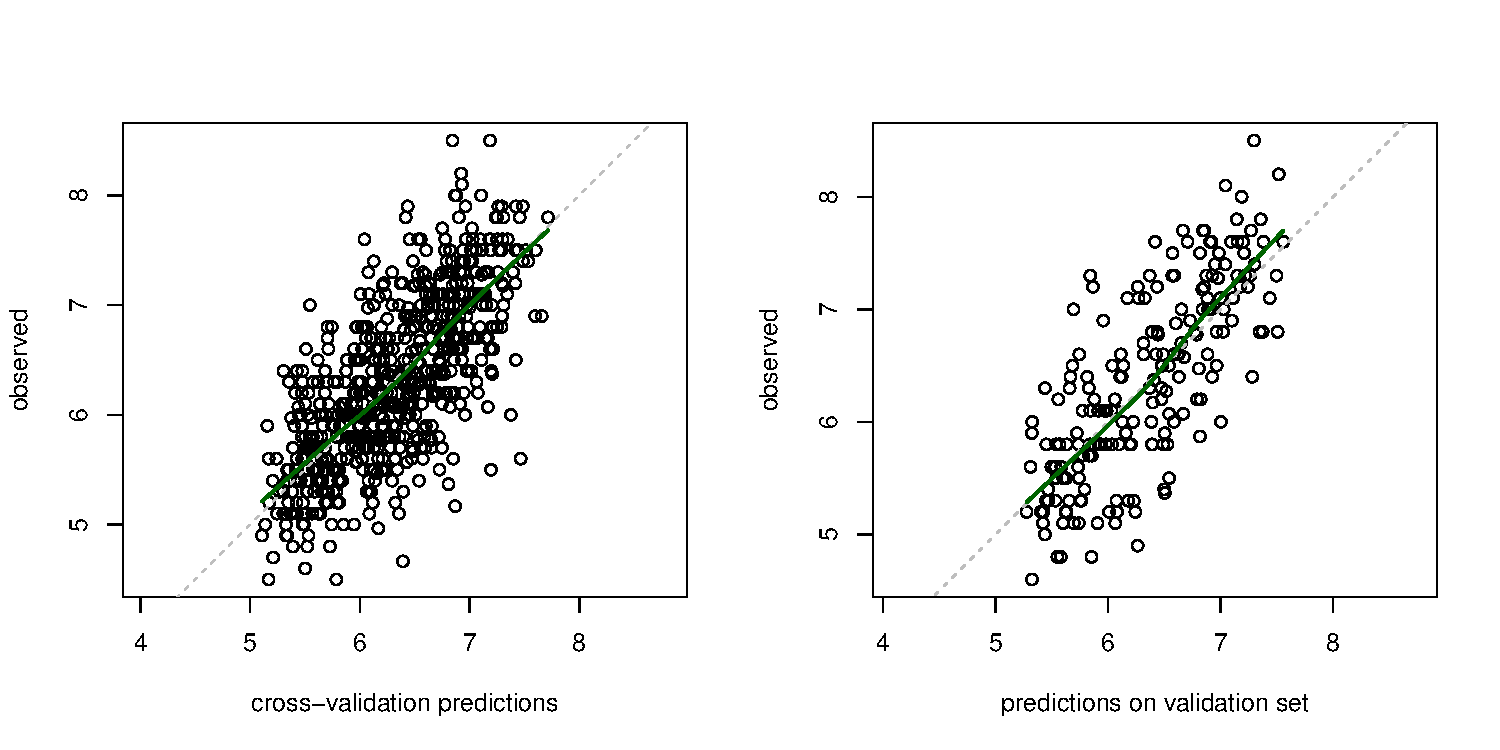
\includegraphics[width=0.85\textwidth]{figure/svm-validation-plots-1} 

}

\caption[Predictions from cross-validation (left) and the validation dataset (right) plotted against the observed values (dashed]{Predictions from cross-validation (left) and the validation dataset (right) plotted against the observed values (dashed: 1:1-line, green: lowess scatterplott smoother).}\label{fig:svm-validation-plots}
\end{figure}


\end{knitrout}


\clearpage 
\section{Random forest}

Here we fit a random forest with the package \texttt{randomForest}. If you work with very large datasets consider using the package \texttt{ranger}. More important: use paralell computing as demonstrated here with the function \texttt{mclapply} (does not work on Windows, then use \texttt{mc.cores = 1}). 

This is advanced programming with functions and \texttt{apply}. But, I wanted to show how you can do the tuning of a ML method yourself without using a meta-function like \texttt{train} from package \texttt{caret} (see below). Like this you can control it does what it should (and the code is not much longer)

\begin{knitrout}
\definecolor{shadecolor}{rgb}{0.969, 0.969, 0.969}\color{fgcolor}\begin{kframe}
\begin{alltt}
\hlcom{# Fit a random forest with default parameters }
\hlcom{# (often results are already quite good)}
\hlkwd{set.seed}\hlstd{(}\hlnum{1}\hlstd{)}
\hlstd{rf.model.basic} \hlkwb{<-} \hlkwd{randomForest}\hlstd{(}\hlkwc{x} \hlstd{= d.ph10[, l.covar ],}
                               \hlkwc{y} \hlstd{= d.ph10[,} \hlstr{"ph.0.10"}\hlstd{])}

\hlcom{# tune main tuning parameter "mtry"}
\hlcom{# (the number of covariates that are randomly selected to try at each split)}

\hlcom{# define function to use below}
\hlstd{f.tune.randomforest} \hlkwb{<-} \hlkwa{function}\hlstd{(}\hlkwc{test.mtry}\hlstd{,} \hlcom{# mtry to test}
                                \hlkwc{d.cal}\hlstd{,}     \hlcom{# calibration data}
                                \hlkwc{l.covariates} \hlstd{)\{} \hlcom{# list of covariates}
  \hlcom{# set seed }
  \hlkwd{set.seed}\hlstd{(}\hlnum{1}\hlstd{)}
  \hlcom{# fit random forest with mtry = test.mtry}
  \hlstd{rf.tune} \hlkwb{<-} \hlkwd{randomForest}\hlstd{(}\hlkwc{x} \hlstd{= d.cal[, l.covariates ],}
                          \hlkwc{y} \hlstd{= d.cal[,} \hlstr{"ph.0.10"}\hlstd{],}
                          \hlkwc{mtry} \hlstd{= test.mtry)}
  \hlcom{# return the mean squared error (mse) of this model fit}
  \hlkwd{return}\hlstd{(} \hlkwd{tail}\hlstd{(rf.tune}\hlopt{$}\hlstd{mse,} \hlkwc{n}\hlstd{=}\hlnum{1}\hlstd{) )}
\hlstd{\}}

\hlcom{# vector of mtry to test }
\hlstd{seq.mtry} \hlkwb{<-} \hlkwd{c}\hlstd{(}\hlnum{1}\hlopt{:}\hlstd{(}\hlkwd{length}\hlstd{(l.covar)} \hlopt{-} \hlnum{1}\hlstd{))}
\hlcom{# Only take every fifth for speed reasons}
\hlstd{seq.mtry} \hlkwb{<-} \hlstd{seq.mtry[ seq.mtry} \hlopt \hlnum{5} \hlopt{==} \hlnum{0} \hlstd{]}

\hlcom{# Apply function to sequence. }
\hlstd{t.OOBe} \hlkwb{<-}   \hlkwd{mclapply}\hlstd{(seq.mtry,} \hlcom{# give sequence }
                     \hlkwc{FUN} \hlstd{= f.tune.randomforest,} \hlcom{# give function name}
                     \hlkwc{mc.cores} \hlstd{=} \hlnum{1}\hlstd{,} \hlcom{## number of CPUs }
                     \hlkwc{mc.set.seed} \hlstd{=} \hlnum{FALSE}\hlstd{,} \hlcom{# do not use new seed each time }
                     \hlcom{# now here giv the arguments to the function:}
                     \hlkwc{d.cal} \hlstd{= d.ph10,}
                     \hlkwc{l.covar} \hlstd{= l.covar )}

\hlcom{# Hint: Who is not comfortable with "mclapply" }
\hlcom{# the same could be achieved with}
\hlcom{# for(test.mtry in 1:m.end)\{ }
\hlcom{#    .. content of function + vector to collect result... \}}

\hlcom{# create a dataframe of the results           }
\hlstd{mtry.oob} \hlkwb{<-} \hlkwd{data.frame}\hlstd{(}\hlkwc{mtry.n} \hlstd{= seq.mtry,} \hlkwc{mtry.OOBe} \hlstd{=} \hlkwd{unlist}\hlstd{(t.OOBe))}

\hlcom{# get the mtry with the minimum MSE}
\hlstd{s.mtry} \hlkwb{<-} \hlstd{mtry.oob}\hlopt{$}\hlstd{mtry.n[} \hlkwd{which.min}\hlstd{(mtry.oob}\hlopt{$}\hlstd{mtry.OOBe) ]}

\hlcom{# compute random forest with optimal mtry }
\hlkwd{set.seed}\hlstd{(}\hlnum{1}\hlstd{)}
\hlstd{rf.model.tuned} \hlkwb{<-} \hlkwd{randomForest}\hlstd{(}\hlkwc{x} \hlstd{= d.ph10[, l.covar ],}
                               \hlkwc{y} \hlstd{= d.ph10[,} \hlstr{"ph.0.10"}\hlstd{],}
                               \hlkwc{mtry} \hlstd{= s.mtry)}
\end{alltt}
\end{kframe}
\end{knitrout}


\begin{knitrout}
\definecolor{shadecolor}{rgb}{0.969, 0.969, 0.969}\color{fgcolor}\begin{kframe}
\begin{alltt}
\hlkwd{plot}\hlstd{( mtry.oob}\hlopt{$}\hlstd{mtry.n, mtry.oob}\hlopt{$}\hlstd{mtry.OOBe,} \hlkwc{pch} \hlstd{=} \hlnum{4}\hlstd{,}
      \hlkwc{ylab} \hlstd{=} \hlstr{"out-of-bag MSE error"}\hlstd{,} \hlkwc{xlab} \hlstd{=} \hlstr{"mtry"}\hlstd{)}
\hlkwd{abline}\hlstd{(}\hlkwc{v} \hlstd{= s.mtry,} \hlkwc{lty} \hlstd{=} \hlstr{"dashed"}\hlstd{,} \hlkwc{col} \hlstd{=} \hlstr{"darkgrey"}\hlstd{)}
\hlkwd{lines}\hlstd{(} \hlkwd{lowess}\hlstd{( mtry.oob}\hlopt{$}\hlstd{mtry.n, mtry.oob}\hlopt{$}\hlstd{mtry.OOBe ),} \hlkwc{lwd} \hlstd{=} \hlnum{1.5}\hlstd{,} \hlkwc{col} \hlstd{=} \hlstr{"darkgrey"}\hlstd{)}
\end{alltt}
\end{kframe}\begin{figure}[!h]

{\centering 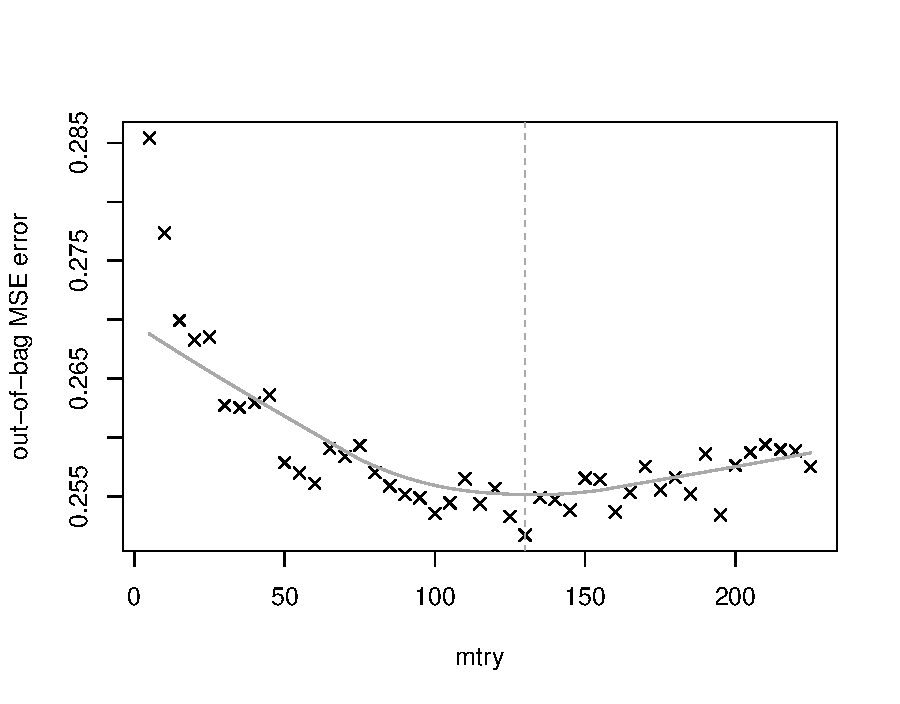
\includegraphics[width=0.6\textwidth]{figure/random-forest-plot-mtry-1} 

}

\caption[Tuning parameter mtry plotted against the out-of-bag mean squared error (grey line]{Tuning parameter mtry plotted against the out-of-bag mean squared error (grey line: lowess smoothing line, dashed line: mtry at minimum MSE).}\label{fig:random-forest-plot-mtry}
\end{figure}


\end{knitrout}


\paragraph{Please continue:}

\begin{itemize}
\item Compute the predictions for the validation set with the tuned and the model with default values (\texttt{predict(rf.model.tuned, newdata = ...)}) and compute a root mean squared error. Was the tuning effort worthwhile? 
\item Implement the same tunging with the package \texttt{caret}. Check the option \texttt{methofd="oob"} of \texttt{trainControl}. This function is handed to \texttt{train}. 
\end{itemize}



\clearpage 
\section{Gradient boosting}

\subsection{Boosting with trees as baselearners}

There are various R packages to fit boosting models (e.g. \texttt{mboost}, \texttt{xgboost}). We use \texttt{gbm} here. We can again tune it with \texttt{caret}. \texttt{caret} is a meta package that provides a homogenous interface to about 80 machine learning methods. 


Fit gradient boosting with trees: 

\begin{knitrout}
\definecolor{shadecolor}{rgb}{0.969, 0.969, 0.969}\color{fgcolor}\begin{kframe}
\begin{alltt}
\hlcom{# create a grid of the tuning parameters to be tested, }
\hlcom{# main tuning parameters are: }
\hlstd{gbm.grid} \hlkwb{<-} \hlkwd{expand.grid}\hlstd{(}
  \hlcom{# how many splits does each tree have}
  \hlkwc{interaction.depth} \hlstd{=} \hlkwd{c}\hlstd{(}\hlnum{2}\hlstd{,}\hlnum{5}\hlstd{,}\hlnum{10}\hlstd{,}\hlnum{15}\hlstd{,}\hlnum{20}\hlstd{),}
  \hlcom{# how many trees do we add (number of iterations of boosting algorithm)}
  \hlkwc{n.trees} \hlstd{=} \hlkwd{seq}\hlstd{(}\hlnum{2}\hlstd{,}\hlnum{250}\hlstd{,} \hlkwc{by} \hlstd{=} \hlnum{5}\hlstd{),}
  \hlcom{# put the shrinkage factor to 0.1 (=10% updates as used }
  \hlcom{# in package mboost), the default (0.1%) is a bit too small, }
  \hlcom{# makes model selection too slow. }
  \hlcom{# minimum number of observations per node can be left as is}
  \hlkwc{shrinkage} \hlstd{=} \hlnum{0.1}\hlstd{,} \hlkwc{n.minobsinnode} \hlstd{=} \hlnum{10}\hlstd{)}

\hlcom{# make tuning reproducible (there are random samples for the cross validation)}
\hlkwd{set.seed}\hlstd{(}\hlnum{291201945}\hlstd{)}

\hlcom{# train the gbm model }
\hlcom{# Remove "ge_caco3" throws an error since Package gbm 2.1.5, }
\hlcom{# this bug is reported: https://github.com/gbm-developers/gbm/issues/40}
\hlstd{gbm.model} \hlkwb{<-} \hlkwd{train}\hlstd{(}\hlkwc{x}\hlstd{=d.ph10[, l.covar[}\hlopt{-}\hlkwd{c}\hlstd{(}\hlnum{50}\hlstd{)]  ],}
                   \hlkwc{y}\hlstd{=d.ph10[,} \hlstr{"ph.0.10"}\hlstd{],}
                   \hlkwc{method} \hlstd{=} \hlstr{"gbm"}\hlstd{,} \hlcom{# choose "generalized boosted regression model"}
                   \hlkwc{tuneGrid} \hlstd{= gbm.grid,}
                   \hlkwc{verbose} \hlstd{=} \hlnum{FALSE}\hlstd{,}
                   \hlkwc{trControl} \hlstd{=} \hlkwd{trainControl}\hlstd{(}
                     \hlcom{# use 10fold cross validation (CV)}
                     \hlkwc{method} \hlstd{=} \hlstr{"cv"}\hlstd{,} \hlkwc{number} \hlstd{=} \hlnum{10}\hlstd{,}
                     \hlcom{# save fitted values (e.g. to calculate RMSE of the CV)}
                     \hlkwc{savePredictions} \hlstd{=} \hlstr{"final"}\hlstd{))}

\hlcom{# print optimal tuning parameter}
\hlstd{gbm.model}\hlopt{$}\hlstd{bestTune}
\end{alltt}
\begin{verbatim}
##    n.trees interaction.depth shrinkage n.minobsinnode
## 24     117                 2       0.1             10
\end{verbatim}
\end{kframe}
\end{knitrout}


\begin{knitrout}
\definecolor{shadecolor}{rgb}{0.969, 0.969, 0.969}\color{fgcolor}\begin{kframe}
\begin{alltt}
\hlcom{# compute predictions for the small part of the study area}
\hlcom{# (agricultural land, the empty pixels are streets, forests etc.)}
\hlkwd{data}\hlstd{(}\hlstr{"berne.grid"}\hlstd{)}

\hlstd{berne.grid}\hlopt{$}\hlstd{pred} \hlkwb{<-} \hlkwd{predict.train}\hlstd{(gbm.model,} \hlkwc{newdata} \hlstd{= berne.grid )}

\hlcom{# create a spatial object for a proper spatial plot}
\hlkwd{coordinates}\hlstd{(berne.grid)} \hlkwb{<-} \hlopt{~}\hlstd{x}\hlopt{+}\hlstd{y}
\hlcom{# add the Swiss projection (see ?berne.grid)}
\hlcom{# see https://epsg.io for details on projections}
\hlkwd{proj4string}\hlstd{(berne.grid)} \hlkwb{<-} \hlkwd{CRS}\hlstd{(}\hlstr{"+init=epsg:21781"}\hlstd{)}
\hlcom{# create a raster object from the spatial point dataframe }
\hlkwd{gridded}\hlstd{(berne.grid)} \hlkwb{<-} \hlnum{TRUE}
\hlkwd{plot}\hlstd{(}\hlkwd{raster}\hlstd{(berne.grid,} \hlkwc{layer} \hlstd{=} \hlstr{"pred"}\hlstd{))}
\end{alltt}
\end{kframe}\begin{figure}

{\centering 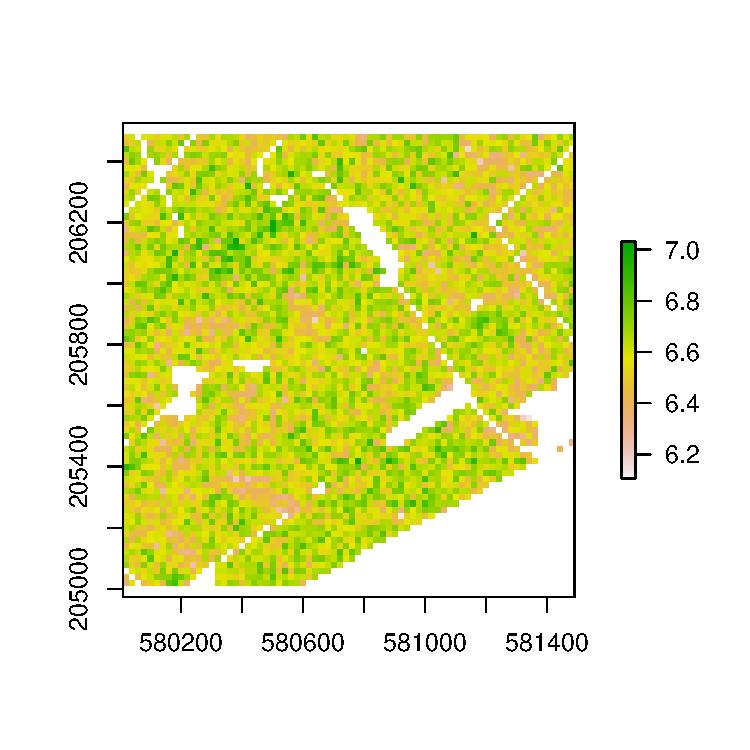
\includegraphics[width=0.7\textwidth]{figure/boosted-trees-map-1} 

}

\caption[Predictions computed with an optimized boosted trees model of topsoil pH (0--10 cm) for a very small part of the Berne study region (white areas are streets, developped areas or forests, CRAN does not accept larger datasets)]{Predictions computed with an optimized boosted trees model of topsoil pH (0--10 cm) for a very small part of the Berne study region (white areas are streets, developped areas or forests, CRAN does not accept larger datasets).}\label{fig:boosted-trees-map}
\end{figure}


\end{knitrout}


Lets check the partial dependencies of the 4 most important covariates: 

\begin{knitrout}
\definecolor{shadecolor}{rgb}{0.969, 0.969, 0.969}\color{fgcolor}\begin{kframe}
\begin{alltt}
\hlcom{# get variable importance}
\hlstd{t.imp} \hlkwb{<-} \hlkwd{varImp}\hlstd{(gbm.model}\hlopt{$}\hlstd{finalModel)}

\hlcom{# check how many covariates were never selected}
\hlkwd{sum}\hlstd{( t.imp}\hlopt{$}\hlstd{Overall} \hlopt{==} \hlnum{0} \hlstd{)}
\end{alltt}
\begin{verbatim}
## [1] 111
\end{verbatim}
\begin{alltt}
\hlcom{# order and select 4 most important covariates}
\hlstd{t.names} \hlkwb{<-} \hlkwd{dimnames}\hlstd{(t.imp)[[}\hlnum{1}\hlstd{]][} \hlkwd{order}\hlstd{(t.imp}\hlopt{$}\hlstd{Overall,} \hlkwc{decreasing} \hlstd{= T)[}\hlnum{1}\hlopt{:}\hlnum{4}\hlstd{] ]}

\hlkwd{par}\hlstd{(}\hlkwc{mfrow} \hlstd{=} \hlkwd{c}\hlstd{(}\hlnum{2}\hlstd{,}\hlnum{2}\hlstd{))}
\hlkwa{for}\hlstd{( name} \hlkwa{in} \hlstd{t.names )\{}
  \hlcom{# select index of covariate}
  \hlstd{ix} \hlkwb{<-} \hlkwd{which}\hlstd{( gbm.model}\hlopt{$}\hlstd{finalModel}\hlopt{$}\hlstd{var.names} \hlopt{==} \hlstd{name )}
  \hlkwd{plot}\hlstd{(gbm.model}\hlopt{$}\hlstd{finalModel,} \hlkwc{i.var} \hlstd{= ix)}
\hlstd{\}}

\hlcom{# -> improve the plots by using the same y-axis (e.g. ylim=c(..,..)) }
\hlcom{#    for all of them, and try to add labels (xlab = , ylab = ) }
\hlcom{#    or a title (main = )}
\end{alltt}
\end{kframe}
\end{knitrout}





\subsection{Boosting with linear baselearners (advanced task)}

Boosting algorithm can be used with any kind of base procedures / baselearners. Many packages (e.g. \texttt{gbm}, \texttt{xgboost}) use trees. Here we try linear and splines baselearners. 


For details on \texttt{mboost} see the hands-on tutorial in the vignette to the package:
\url{https://cran.r-project.org/web/packages/mboost/vignettes/mboost_tutorial.pdf}

Select a boosting model with linear baselearners (this results in shrunken coefficients, similar to the lasso, see Hastie et al. 2009): 

\begin{knitrout}
\definecolor{shadecolor}{rgb}{0.969, 0.969, 0.969}\color{fgcolor}\begin{kframe}
\begin{alltt}
\hlcom{# Fit model}
\hlstd{ph.glmboost} \hlkwb{<-} \hlkwd{glmboost}\hlstd{(ph.0.10} \hlopt{~}\hlstd{.,} \hlkwc{data} \hlstd{= d.ph10[} \hlkwd{c}\hlstd{(}\hlstr{"ph.0.10"}\hlstd{, l.covar)],}
                        \hlkwc{control} \hlstd{=} \hlkwd{boost_control}\hlstd{(}\hlkwc{mstop} \hlstd{=} \hlnum{200}\hlstd{),}
                        \hlkwc{center} \hlstd{=} \hlnum{TRUE}\hlstd{)}

\hlcom{# Find tuning parameter: mstop = number of boosting itertations}
\hlkwd{set.seed}\hlstd{(}\hlnum{42}\hlstd{)}
\hlstd{ph.glmboost.cv} \hlkwb{<-} \hlkwd{cvrisk}\hlstd{(ph.glmboost,}
                         \hlkwc{folds} \hlstd{= mboost}\hlopt{::}\hlkwd{cv}\hlstd{(}\hlkwd{model.weights}\hlstd{(ph.glmboost),}
                                            \hlkwc{type} \hlstd{=} \hlstr{"kfold"}\hlstd{))}

\hlcom{# print optimal mstop}
\hlkwd{mstop}\hlstd{(ph.glmboost.cv)}
\end{alltt}
\begin{verbatim}
## [1] 96
\end{verbatim}
\begin{alltt}
\hlcom{## print model with fitted coefficents }
\hlcom{# ph.glmboost[ mstop(ph.glmboost.cv)]}
\end{alltt}
\end{kframe}
\end{knitrout}


\begin{knitrout}
\definecolor{shadecolor}{rgb}{0.969, 0.969, 0.969}\color{fgcolor}\begin{figure}

{\centering 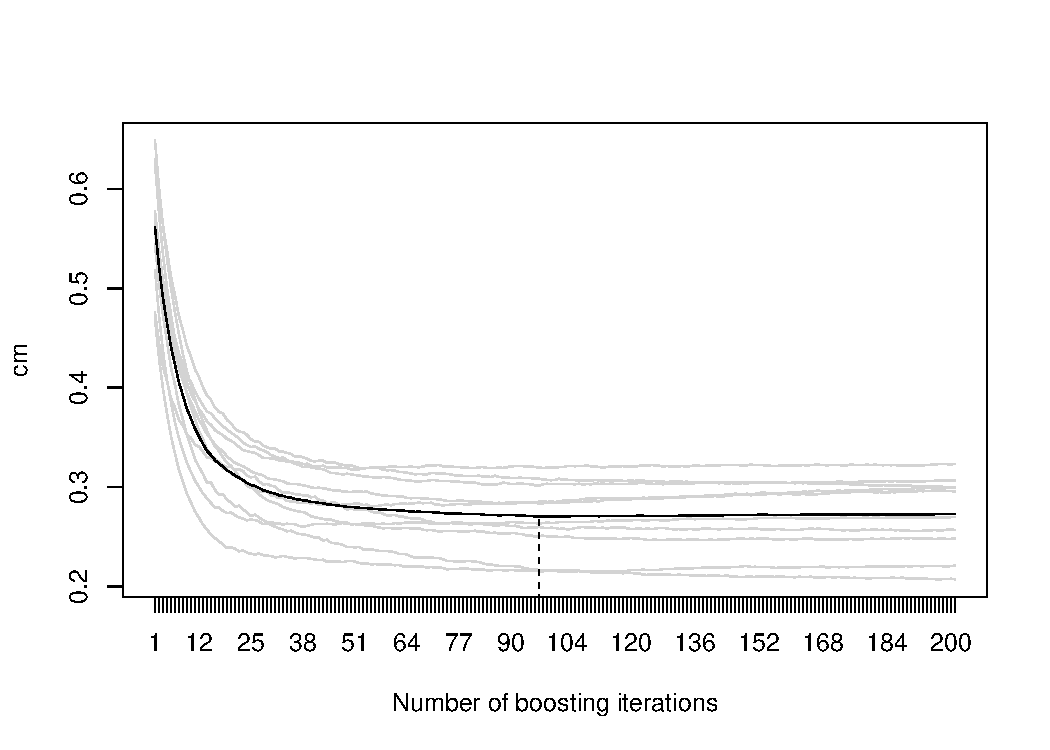
\includegraphics[width=0.8\textwidth]{figure/glmboost-plot-1} 

}

\caption[Path of cross validation error along the boosting iterations]{Path of cross validation error along the boosting iterations.}\label{fig:glmboost-plot}
\end{figure}


\end{knitrout}


\subsection{Boosting with splines baselearners (advanced task)}

To model non-linear relationships we use splines baselearners. Spatial autocorrelation can be captured by adding a smooth spatial surface. This type of model needs a bit more setup. Each covariate type has its own specification. All baselearners should have the same degrees of freedom, otherwise biased model selection might be the result.  

\begin{knitrout}
\definecolor{shadecolor}{rgb}{0.969, 0.969, 0.969}\color{fgcolor}\begin{kframe}
\begin{alltt}
\hlcom{# quick set up formula}

\hlcom{# Response}
\hlstd{f.resp} \hlkwb{<-} \hlstr{"ph.0.10 ~ "}

\hlcom{# Intercept, add to dataframe }
\hlstd{f.int} \hlkwb{<-} \hlstr{"bols(int, intercept = F, df = 1)"}
\hlstd{d.ph10}\hlopt{$}\hlstd{int} \hlkwb{<-} \hlkwd{rep}\hlstd{(}\hlnum{1}\hlstd{,} \hlkwd{nrow}\hlstd{(d.ph10))}

\hlcom{# Smooth spatial surface (needs > 4 degrees of freedom)}
\hlstd{f.spat} \hlkwb{<-} \hlstr{"bspatial(x, y, df = 5, knots = 12)"}

\hlcom{# Linear baselearners for factors, maybe use df = 5}
\hlstd{f.fact} \hlkwb{<-} \hlkwd{paste}\hlstd{(}
  \hlkwd{paste}\hlstd{(} \hlstr{"bols("}\hlstd{, l.factors,} \hlstr{", intercept = F)"} \hlstd{),}
  \hlkwc{collapse} \hlstd{=} \hlstr{"+"}
\hlstd{)}

\hlcom{# Splines baselearners for continuous covariates}
\hlstd{f.num} \hlkwb{<-} \hlkwd{paste}\hlstd{(}
  \hlkwd{paste}\hlstd{(} \hlstr{"bbs("}\hlstd{, l.numeric,} \hlstr{", center = T, df = 5)"} \hlstd{),}
  \hlkwc{collapse} \hlstd{=} \hlstr{"+"}
\hlstd{)}

\hlcom{# create complete formula }
\hlstd{ph.form} \hlkwb{<-} \hlkwd{as.formula}\hlstd{(} \hlkwd{paste}\hlstd{( f.resp,}
                              \hlkwd{paste}\hlstd{(} \hlkwd{c}\hlstd{(f.int, f.num, f.spat, f.fact),}
                                     \hlkwc{collapse} \hlstd{=} \hlstr{"+"}\hlstd{)) )}
\hlcom{# fit the boosting model}
\hlstd{ph.gamboost}  \hlkwb{<-} \hlkwd{gamboost}\hlstd{(ph.form,} \hlkwc{data} \hlstd{= d.ph10,}
                         \hlkwc{control} \hlstd{=} \hlkwd{boost_control}\hlstd{(}\hlkwc{mstop} \hlstd{=} \hlnum{200}\hlstd{))}

\hlcom{# Find tuning parameter}
\hlstd{ph.gamboost.cv} \hlkwb{<-} \hlkwd{cvrisk}\hlstd{(ph.gamboost,}
                         \hlkwc{folds} \hlstd{= mboost}\hlopt{::}\hlkwd{cv}\hlstd{(}\hlkwd{model.weights}\hlstd{(ph.gamboost),}
                                            \hlkwc{type} \hlstd{=} \hlstr{"kfold"}\hlstd{))}
\end{alltt}
\end{kframe}
\end{knitrout}

Analyse boosting model:

\begin{knitrout}
\definecolor{shadecolor}{rgb}{0.969, 0.969, 0.969}\color{fgcolor}\begin{kframe}
\begin{alltt}
\hlcom{# print optimal mstop}
\hlkwd{mstop}\hlstd{(ph.gamboost.cv)}
\end{alltt}
\begin{verbatim}
## [1] 192
\end{verbatim}
\begin{alltt}
\hlcom{## print model info }
\hlstd{ph.gamboost[} \hlkwd{mstop}\hlstd{(ph.glmboost.cv)]}
\end{alltt}
\begin{verbatim}
## 
## 	 Model-based Boosting
## 
## Call:
## gamboost(formula = ph.form, data = d.ph10, control = boost_control(mstop = 200))
## 
## 
## 	 Squared Error (Regression) 
## 
## Loss function: (y - f)^2 
##  
## 
## Number of boosting iterations: mstop = 96 
## Step size:  0.1 
## Offset:  6.314042 
## Number of baselearners:  228
\end{verbatim}
\begin{alltt}
\hlcom{## print number of chosen baselearners }
\hlkwd{length}\hlstd{( t.sel} \hlkwb{<-}  \hlkwd{summary}\hlstd{( ph.gamboost[} \hlkwd{mstop}\hlstd{(ph.glmboost.cv)] )}\hlopt{$}\hlstd{selprob )}
\end{alltt}
\begin{verbatim}
## [1] 33
\end{verbatim}
\begin{alltt}
\hlcom{# Most often selected were: }
\hlkwd{summary}\hlstd{( ph.gamboost[} \hlkwd{mstop}\hlstd{(ph.glmboost.cv)] )}\hlopt{$}\hlstd{selprob[}\hlnum{1}\hlopt{:}\hlnum{5}\hlstd{]}
\end{alltt}
\begin{verbatim}
##                    bols(timeset, intercept = F) 
##                                      0.14583333 
##             bbs(cl_mt_gh_3, df = 5, center = T) 
##                                      0.08333333 
##         bbs(tr_ch_3_80_10s, df = 5, center = T) 
##                                      0.06250000 
##             bbs(cl_mt_gh_8, df = 5, center = T) 
##                                      0.05208333 
## bbs(tr_be_twi2m_s60_tcilow, df = 5, center = T) 
##                                      0.05208333
\end{verbatim}
\end{kframe}
\end{knitrout}

\begin{knitrout}
\definecolor{shadecolor}{rgb}{0.969, 0.969, 0.969}\color{fgcolor}\begin{figure}

{\centering 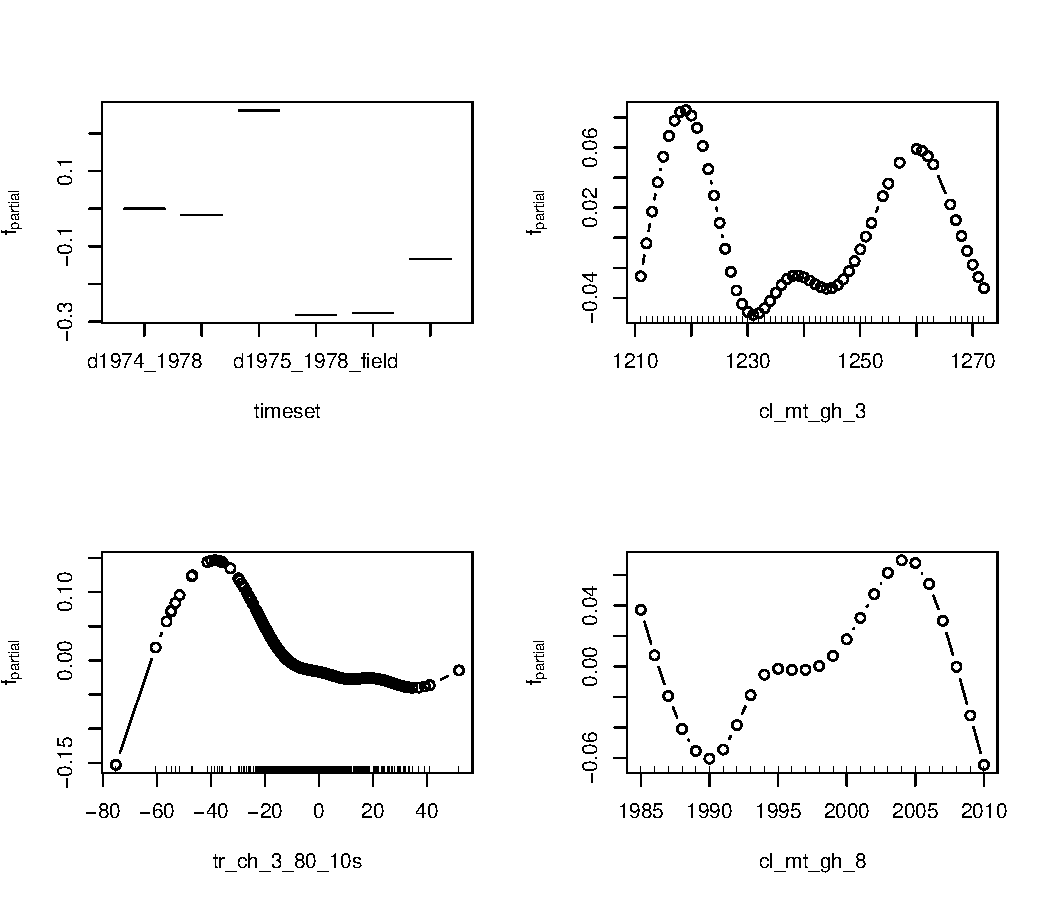
\includegraphics[width=0.8\textwidth]{figure/gamboost-partial-plots-1} 

}

\caption[Residual plots of the 4 covariates with highest selection frequency]{Residual plots of the 4 covariates with highest selection frequency.}\label{fig:gamboost-partial-plots}
\end{figure}


\end{knitrout}

\begin{knitrout}
\definecolor{shadecolor}{rgb}{0.969, 0.969, 0.969}\color{fgcolor}\begin{figure}

{\centering 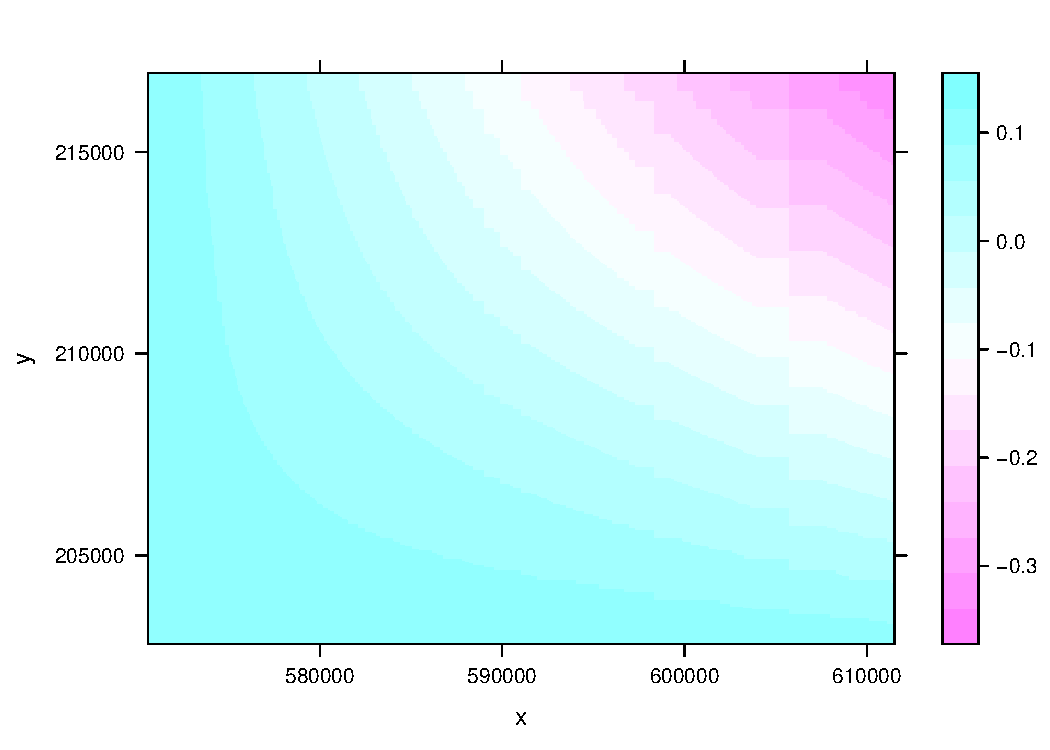
\includegraphics[width=0.8\textwidth]{figure/gamboost-partial-plots-spatial-1} 

}

\caption[Modelled smooth spatial surface based on the coordinates]{Modelled smooth spatial surface based on the coordinates.}\label{fig:gamboost-partial-plots-spatial}
\end{figure}


\end{knitrout}

\clearpage


\section{Model averaging}

So far we calibrated several models to predict topsoil pH. With model averaging we can combine these predictions computing a simple \texttt{mean}. Besides simple averaging, we could use weights like $\frac{1}{MSE}$ (make sure they sum up to 1). 

Compute validation statistics (e.g. root mean squared error, R$^2$) on the validation set for the predictions of each model and the (weighted) averaged predictions. Is the prediction accuracy improved?

You could now add models computed from random forest, support vector machines or gradient boosted trees. Does this improve model accuracy?

\bigskip

Note: Be aware not to select the final model based on the validation data. If you start tuning your predictions on your validation data, you loose the independent estimate of prediction accuracy... better choose your method for the final predictions based on cross validation (e.g. on the same sets).  




\bigskip 
\section*{R session information}

\footnotesize
This document was generated with:
\begin{kframe}
\begin{alltt}
\hlkwd{toLatex}\hlstd{(}\hlkwd{sessionInfo}\hlstd{(),} \hlkwc{locale} \hlstd{=} \hlnum{FALSE}\hlstd{)}
\end{alltt}
\end{kframe}\begin{itemize}\raggedright
  \item R version 3.6.3 (2020-02-29), \verb|x86_64-pc-linux-gnu|
  \item Running under: \verb|Progress Linux 5+ (engywuck-backports)|
  \item Matrix products: default
  \item BLAS:   \verb|/usr/lib/x86_64-linux-gnu/openblas/libblas.so.3|
  \item LAPACK: \verb|/usr/lib/x86_64-linux-gnu/libopenblasp-r0.3.5.so|
  \item Base packages: base, datasets, graphics, grDevices, methods,
    parallel, stats, utils
  \item Other packages: caret~6.0-85, gbm~2.1.5, geoGAM~0.1-2,
    ggplot2~3.2.1, glmnet~3.0-2, grpreg~3.2-1, kernlab~0.9-29,
    knitr~1.27, lattice~0.20-38, Matrix~1.2-18, mboost~2.9-1,
    randomForest~4.6-14, raster~3.0-7, sp~1.3-2, stabs~0.6-3
  \item Loaded via a namespace (and not attached): assertthat~0.2.1,
    class~7.3-15, codetools~0.2-16, colorspace~1.4-1, compiler~3.6.3,
    crayon~1.3.4, data.table~1.12.8, digest~0.6.23, dplyr~0.8.3,
    evaluate~0.14, foreach~1.4.7, Formula~1.2-3, generics~0.0.2,
    glue~1.3.1, gower~0.2.1, grid~3.6.3, gridExtra~2.3, gtable~0.3.0,
    highr~0.8, inum~1.0-1, ipred~0.9-9, iterators~1.0.12, lava~1.6.6,
    lazyeval~0.2.2, libcoin~1.0-5, lifecycle~0.1.0, lubridate~1.7.4,
    magrittr~1.5, MASS~7.3-51.5, mgcv~1.8-31, ModelMetrics~1.2.2.1,
    munsell~0.5.0, mvtnorm~1.0-12, nlme~3.1-143, nnet~7.3-12, nnls~1.4,
    partykit~1.2-5, pillar~1.4.3, pkgconfig~2.0.3, plyr~1.8.5,
    pROC~1.16.1, prodlim~2019.11.13, purrr~0.3.3, quadprog~1.5-8,
    R6~2.4.1, Rcpp~1.0.3, recipes~0.1.9, reshape2~1.4.3, rgdal~1.4-8,
    rlang~0.4.2, rpart~4.1-15, scales~1.1.0, shape~1.4.4,
    splines~3.6.3, stats4~3.6.3, stringi~1.4.5, stringr~1.4.0,
    survival~3.1-8, tibble~2.1.3, tidyselect~0.2.5, timeDate~3043.102,
    tools~3.6.3, withr~2.1.2, xfun~0.12
\end{itemize}

\normalsize




\end{document}
